% Graphic for TeX using PGF
% Title: S:\Senior Project\seniorProject2-2020-21-Docs\figs\dia\algorithmFlowchart.dia
% Creator: Dia v0.97.2
% CreationDate: Thu Nov 19 16:57:28 2020
% For: Jason Braker
% \usepackage{tikz}
% The following commands are not supported in PSTricks at present
% We define them conditionally, so when they are implemented,
% this pgf file will use them.
\ifx\du\undefined
  \newlength{\du}
\fi
\setlength{\du}{15\unitlength}
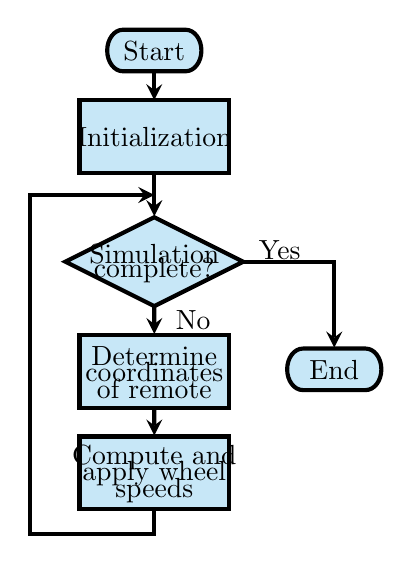
\begin{tikzpicture}[scale=0.5]
\pgftransformxscale{1.000000}
\pgftransformyscale{-1.000000}
\definecolor{dialinecolor}{rgb}{0.000000, 0.000000, 0.000000}
\pgfsetstrokecolor{dialinecolor}
\definecolor{dialinecolor}{rgb}{1.000000, 1.000000, 1.000000}
\pgfsetfillcolor{dialinecolor}
\pgfsetlinewidth{0.100000\du}
\pgfsetdash{}{0pt}
\pgfsetdash{}{0pt}
\pgfsetbuttcap
\pgfsetmiterjoin
\pgfsetlinewidth{0.100000\du}
\pgfsetbuttcap
\pgfsetmiterjoin
\pgfsetdash{}{0pt}
\definecolor{dialinecolor}{rgb}{0.780392, 0.905882, 0.968627}
\pgfsetfillcolor{dialinecolor}
\pgfpathmoveto{\pgfpoint{18.786863\du}{3.950000\du}}
\pgfpathlineto{\pgfpoint{21.813113\du}{3.950000\du}}
\pgfpathcurveto{\pgfpoint{22.230951\du}{3.950000\du}}{\pgfpoint{22.569675\du}{4.397715\du}}{\pgfpoint{22.569675\du}{4.950000\du}}
\pgfpathcurveto{\pgfpoint{22.569675\du}{5.502285\du}}{\pgfpoint{22.230951\du}{5.950000\du}}{\pgfpoint{21.813113\du}{5.950000\du}}
\pgfpathlineto{\pgfpoint{18.786863\du}{5.950000\du}}
\pgfpathcurveto{\pgfpoint{18.369024\du}{5.950000\du}}{\pgfpoint{18.030300\du}{5.502285\du}}{\pgfpoint{18.030300\du}{4.950000\du}}
\pgfpathcurveto{\pgfpoint{18.030300\du}{4.397715\du}}{\pgfpoint{18.369024\du}{3.950000\du}}{\pgfpoint{18.786863\du}{3.950000\du}}
\pgfusepath{fill}
\definecolor{dialinecolor}{rgb}{0.000000, 0.000000, 0.000000}
\pgfsetstrokecolor{dialinecolor}
\pgfpathmoveto{\pgfpoint{18.786863\du}{3.950000\du}}
\pgfpathlineto{\pgfpoint{21.813113\du}{3.950000\du}}
\pgfpathcurveto{\pgfpoint{22.230951\du}{3.950000\du}}{\pgfpoint{22.569675\du}{4.397715\du}}{\pgfpoint{22.569675\du}{4.950000\du}}
\pgfpathcurveto{\pgfpoint{22.569675\du}{5.502285\du}}{\pgfpoint{22.230951\du}{5.950000\du}}{\pgfpoint{21.813113\du}{5.950000\du}}
\pgfpathlineto{\pgfpoint{18.786863\du}{5.950000\du}}
\pgfpathcurveto{\pgfpoint{18.369024\du}{5.950000\du}}{\pgfpoint{18.030300\du}{5.502285\du}}{\pgfpoint{18.030300\du}{4.950000\du}}
\pgfpathcurveto{\pgfpoint{18.030300\du}{4.397715\du}}{\pgfpoint{18.369024\du}{3.950000\du}}{\pgfpoint{18.786863\du}{3.950000\du}}
\pgfusepath{stroke}
% setfont left to latex
\definecolor{dialinecolor}{rgb}{0.000000, 0.000000, 0.000000}
\pgfsetstrokecolor{dialinecolor}
\node at (20.299988\du,4.990000\du){Start};
\definecolor{dialinecolor}{rgb}{0.780392, 0.905882, 0.968627}
\pgfsetfillcolor{dialinecolor}
\fill (16.698800\du,18.658900\du)--(16.698800\du,22.158900\du)--(23.901300\du,22.158900\du)--(23.901300\du,18.658900\du)--cycle;
\pgfsetlinewidth{0.100000\du}
\pgfsetdash{}{0pt}
\pgfsetdash{}{0pt}
\pgfsetmiterjoin
\definecolor{dialinecolor}{rgb}{0.000000, 0.000000, 0.000000}
\pgfsetstrokecolor{dialinecolor}
\draw (16.698800\du,18.658900\du)--(16.698800\du,22.158900\du)--(23.901300\du,22.158900\du)--(23.901300\du,18.658900\du)--cycle;
% setfont left to latex
\definecolor{dialinecolor}{rgb}{0.000000, 0.000000, 0.000000}
\pgfsetstrokecolor{dialinecolor}
\node at (20.300050\du,19.648900\du){Determine};
% setfont left to latex
\definecolor{dialinecolor}{rgb}{0.000000, 0.000000, 0.000000}
\pgfsetstrokecolor{dialinecolor}
\node at (20.300050\du,20.448900\du){coordinates};
% setfont left to latex
\definecolor{dialinecolor}{rgb}{0.000000, 0.000000, 0.000000}
\pgfsetstrokecolor{dialinecolor}
\node at (20.300050\du,21.248900\du){of remote};
\definecolor{dialinecolor}{rgb}{0.780392, 0.905882, 0.968627}
\pgfsetfillcolor{dialinecolor}
\fill (16.698700\du,7.341080\du)--(16.698700\du,10.841080\du)--(23.901200\du,10.841080\du)--(23.901200\du,7.341080\du)--cycle;
\pgfsetlinewidth{0.100000\du}
\pgfsetdash{}{0pt}
\pgfsetdash{}{0pt}
\pgfsetmiterjoin
\definecolor{dialinecolor}{rgb}{0.000000, 0.000000, 0.000000}
\pgfsetstrokecolor{dialinecolor}
\draw (16.698700\du,7.341080\du)--(16.698700\du,10.841080\du)--(23.901200\du,10.841080\du)--(23.901200\du,7.341080\du)--cycle;
% setfont left to latex
\definecolor{dialinecolor}{rgb}{0.000000, 0.000000, 0.000000}
\pgfsetstrokecolor{dialinecolor}
\node at (20.299950\du,9.131080\du){Initialization};
\definecolor{dialinecolor}{rgb}{0.780392, 0.905882, 0.968627}
\pgfsetfillcolor{dialinecolor}
\fill (16.698700\du,23.550000\du)--(16.698700\du,27.050000\du)--(23.901200\du,27.050000\du)--(23.901200\du,23.550000\du)--cycle;
\pgfsetlinewidth{0.100000\du}
\pgfsetdash{}{0pt}
\pgfsetdash{}{0pt}
\pgfsetmiterjoin
\definecolor{dialinecolor}{rgb}{0.000000, 0.000000, 0.000000}
\pgfsetstrokecolor{dialinecolor}
\draw (16.698700\du,23.550000\du)--(16.698700\du,27.050000\du)--(23.901200\du,27.050000\du)--(23.901200\du,23.550000\du)--cycle;
% setfont left to latex
\definecolor{dialinecolor}{rgb}{0.000000, 0.000000, 0.000000}
\pgfsetstrokecolor{dialinecolor}
\node at (20.299950\du,24.540000\du){Compute and};
% setfont left to latex
\definecolor{dialinecolor}{rgb}{0.000000, 0.000000, 0.000000}
\pgfsetstrokecolor{dialinecolor}
\node at (20.299950\du,25.340000\du){apply wheel};
% setfont left to latex
\definecolor{dialinecolor}{rgb}{0.000000, 0.000000, 0.000000}
\pgfsetstrokecolor{dialinecolor}
\node at (20.299950\du,26.140000\du){speeds};
\definecolor{dialinecolor}{rgb}{0.780392, 0.905882, 0.968627}
\pgfsetfillcolor{dialinecolor}
\fill (20.299960\du,12.982200\du)--(24.585620\du,15.125030\du)--(20.299960\du,17.267860\du)--(16.014300\du,15.125030\du)--cycle;
\pgfsetlinewidth{0.100000\du}
\pgfsetdash{}{0pt}
\pgfsetdash{}{0pt}
\pgfsetmiterjoin
\definecolor{dialinecolor}{rgb}{0.000000, 0.000000, 0.000000}
\pgfsetstrokecolor{dialinecolor}
\draw (20.299960\du,12.982200\du)--(24.585620\du,15.125030\du)--(20.299960\du,17.267860\du)--(16.014300\du,15.125030\du)--cycle;
% setfont left to latex
\definecolor{dialinecolor}{rgb}{0.000000, 0.000000, 0.000000}
\pgfsetstrokecolor{dialinecolor}
\node at (20.299960\du,14.765030\du){Simulation};
% setfont left to latex
\definecolor{dialinecolor}{rgb}{0.000000, 0.000000, 0.000000}
\pgfsetstrokecolor{dialinecolor}
\node at (20.299960\du,15.565030\du){complete?};
\pgfsetlinewidth{0.100000\du}
\pgfsetdash{}{0pt}
\pgfsetdash{}{0pt}
\pgfsetbuttcap
\pgfsetmiterjoin
\pgfsetlinewidth{0.100000\du}
\pgfsetbuttcap
\pgfsetmiterjoin
\pgfsetdash{}{0pt}
\definecolor{dialinecolor}{rgb}{0.780392, 0.905882, 0.968627}
\pgfsetfillcolor{dialinecolor}
\pgfpathmoveto{\pgfpoint{27.457863\du}{19.310600\du}}
\pgfpathlineto{\pgfpoint{30.484113\du}{19.310600\du}}
\pgfpathcurveto{\pgfpoint{30.901951\du}{19.310600\du}}{\pgfpoint{31.240675\du}{19.758315\du}}{\pgfpoint{31.240675\du}{20.310600\du}}
\pgfpathcurveto{\pgfpoint{31.240675\du}{20.862885\du}}{\pgfpoint{30.901951\du}{21.310600\du}}{\pgfpoint{30.484113\du}{21.310600\du}}
\pgfpathlineto{\pgfpoint{27.457863\du}{21.310600\du}}
\pgfpathcurveto{\pgfpoint{27.040024\du}{21.310600\du}}{\pgfpoint{26.701300\du}{20.862885\du}}{\pgfpoint{26.701300\du}{20.310600\du}}
\pgfpathcurveto{\pgfpoint{26.701300\du}{19.758315\du}}{\pgfpoint{27.040024\du}{19.310600\du}}{\pgfpoint{27.457863\du}{19.310600\du}}
\pgfusepath{fill}
\definecolor{dialinecolor}{rgb}{0.000000, 0.000000, 0.000000}
\pgfsetstrokecolor{dialinecolor}
\pgfpathmoveto{\pgfpoint{27.457863\du}{19.310600\du}}
\pgfpathlineto{\pgfpoint{30.484113\du}{19.310600\du}}
\pgfpathcurveto{\pgfpoint{30.901951\du}{19.310600\du}}{\pgfpoint{31.240675\du}{19.758315\du}}{\pgfpoint{31.240675\du}{20.310600\du}}
\pgfpathcurveto{\pgfpoint{31.240675\du}{20.862885\du}}{\pgfpoint{30.901951\du}{21.310600\du}}{\pgfpoint{30.484113\du}{21.310600\du}}
\pgfpathlineto{\pgfpoint{27.457863\du}{21.310600\du}}
\pgfpathcurveto{\pgfpoint{27.040024\du}{21.310600\du}}{\pgfpoint{26.701300\du}{20.862885\du}}{\pgfpoint{26.701300\du}{20.310600\du}}
\pgfpathcurveto{\pgfpoint{26.701300\du}{19.758315\du}}{\pgfpoint{27.040024\du}{19.310600\du}}{\pgfpoint{27.457863\du}{19.310600\du}}
\pgfusepath{stroke}
% setfont left to latex
\definecolor{dialinecolor}{rgb}{0.000000, 0.000000, 0.000000}
\pgfsetstrokecolor{dialinecolor}
\node at (28.970988\du,20.350600\du){End};
\pgfsetlinewidth{0.100000\du}
\pgfsetdash{}{0pt}
\pgfsetdash{}{0pt}
\pgfsetbuttcap
{
\definecolor{dialinecolor}{rgb}{0.000000, 0.000000, 0.000000}
\pgfsetfillcolor{dialinecolor}
% was here!!!
\pgfsetarrowsend{stealth}
\definecolor{dialinecolor}{rgb}{0.000000, 0.000000, 0.000000}
\pgfsetstrokecolor{dialinecolor}
\draw (20.300000\du,5.950000\du)--(20.300000\du,7.341080\du);
}
\pgfsetlinewidth{0.100000\du}
\pgfsetdash{}{0pt}
\pgfsetdash{}{0pt}
\pgfsetbuttcap
{
\definecolor{dialinecolor}{rgb}{0.000000, 0.000000, 0.000000}
\pgfsetfillcolor{dialinecolor}
% was here!!!
\pgfsetarrowsend{stealth}
\definecolor{dialinecolor}{rgb}{0.000000, 0.000000, 0.000000}
\pgfsetstrokecolor{dialinecolor}
\draw (20.299953\du,10.889775\du)--(20.299956\du,12.932202\du);
}
\pgfsetlinewidth{0.100000\du}
\pgfsetdash{}{0pt}
\pgfsetdash{}{0pt}
\pgfsetbuttcap
{
\definecolor{dialinecolor}{rgb}{0.000000, 0.000000, 0.000000}
\pgfsetfillcolor{dialinecolor}
% was here!!!
\pgfsetarrowsend{stealth}
\definecolor{dialinecolor}{rgb}{0.000000, 0.000000, 0.000000}
\pgfsetstrokecolor{dialinecolor}
\draw (20.299997\du,17.317846\du)--(20.300019\du,18.610630\du);
}
\pgfsetlinewidth{0.100000\du}
\pgfsetdash{}{0pt}
\pgfsetdash{}{0pt}
\pgfsetbuttcap
{
\definecolor{dialinecolor}{rgb}{0.000000, 0.000000, 0.000000}
\pgfsetfillcolor{dialinecolor}
% was here!!!
\pgfsetarrowsend{stealth}
\definecolor{dialinecolor}{rgb}{0.000000, 0.000000, 0.000000}
\pgfsetstrokecolor{dialinecolor}
\draw (20.300013\du,22.207239\du)--(20.299987\du,23.501661\du);
}
\pgfsetlinewidth{0.100000\du}
\pgfsetdash{}{0pt}
\pgfsetdash{}{0pt}
\pgfsetmiterjoin
\pgfsetbuttcap
{
\definecolor{dialinecolor}{rgb}{0.000000, 0.000000, 0.000000}
\pgfsetfillcolor{dialinecolor}
% was here!!!
\pgfsetarrowsend{stealth}
{\pgfsetcornersarced{\pgfpoint{0.000000\du}{0.000000\du}}\definecolor{dialinecolor}{rgb}{0.000000, 0.000000, 0.000000}
\pgfsetstrokecolor{dialinecolor}
\draw (20.300000\du,27.050000\du)--(20.300000\du,28.250000\du)--(14.300000\du,28.250000\du)--(14.300000\du,11.911000\du)--(20.300000\du,11.911000\du);
}}
\pgfsetlinewidth{0.100000\du}
\pgfsetdash{}{0pt}
\pgfsetdash{}{0pt}
\pgfsetmiterjoin
\pgfsetbuttcap
{
\definecolor{dialinecolor}{rgb}{0.000000, 0.000000, 0.000000}
\pgfsetfillcolor{dialinecolor}
% was here!!!
\pgfsetarrowsend{stealth}
{\pgfsetcornersarced{\pgfpoint{0.000000\du}{0.000000\du}}\definecolor{dialinecolor}{rgb}{0.000000, 0.000000, 0.000000}
\pgfsetstrokecolor{dialinecolor}
\draw (24.585700\du,15.125000\du)--(24.585700\du,15.151500\du)--(28.970990\du,15.151500\du)--(28.970988\du,19.261398\du);
}}
% setfont left to latex
\definecolor{dialinecolor}{rgb}{0.000000, 0.000000, 0.000000}
\pgfsetstrokecolor{dialinecolor}
\node[anchor=west] at (24.800000\du,14.550000\du){Yes};
% setfont left to latex
\definecolor{dialinecolor}{rgb}{0.000000, 0.000000, 0.000000}
\pgfsetstrokecolor{dialinecolor}
\node[anchor=west] at (20.797500\du,17.925000\du){No};
\end{tikzpicture}
